%%% Ne pas modifier jusqu'à la ligne 25
\documentclass[a4paper,12pt]{book}
\usepackage[utf8]{inputenc}
\usepackage[french]{babel}
%%\usepackage{CJK}
\usepackage{yhmath}
\usepackage[left=2cm,right=2cm,top=3cm,bottom=2cm, headheight=1.5cm,headsep=1.5cm]{geometry}
%%\usepackage{CJKutf8}
\usepackage{amsfonts}
\usepackage{mathrsfs}
\usepackage{amsmath,amsfonts,amssymb,dsfont}
\usepackage{graphicx}
\usepackage{subfigure}
\usepackage{enumitem}		%\enumerate-resume
\usepackage[colorlinks=true,unicode={true},hyperindex=false, linkcolor=blue, urlcolor=blue]{hyperref}
\newcommand{\myref}[1]{\ref{#1} page \pageref{#1}}

\addto\captionsfrench{\def\tablename{Tableau}}  %légendes des tableaux
\renewcommand\thesection{\Roman{section}~-~} 
\renewcommand\thesubsection{\Roman{section}.\Alph{subsection}~-~} 
\renewcommand\thesubsubsection{\Roman{section}.\Alph{subsection}.\arabic{subsubsection}~-~} 

\newcommand{\conclusion}[1]{\newline \centerline{\fbox{#1}}}

\setcounter{secnumdepth}{3}
\parindent=0pt

\usepackage{fancyhdr}
\pagestyle{fancy}

\lhead{SJTU-ParisTech} 
%%%%%%%%%%%%%%%%%%%%%%%%%%%%%%%%%%
\chead{TR13}
\rhead{Daniel 518261910024}

\begin{document}
\renewcommand{\labelitemi}{$\blacktriangleright$}
\renewcommand{\labelitemii}{$\bullet$}


\section{réseau}
\begin{figure}[h]
    \begin{center}
    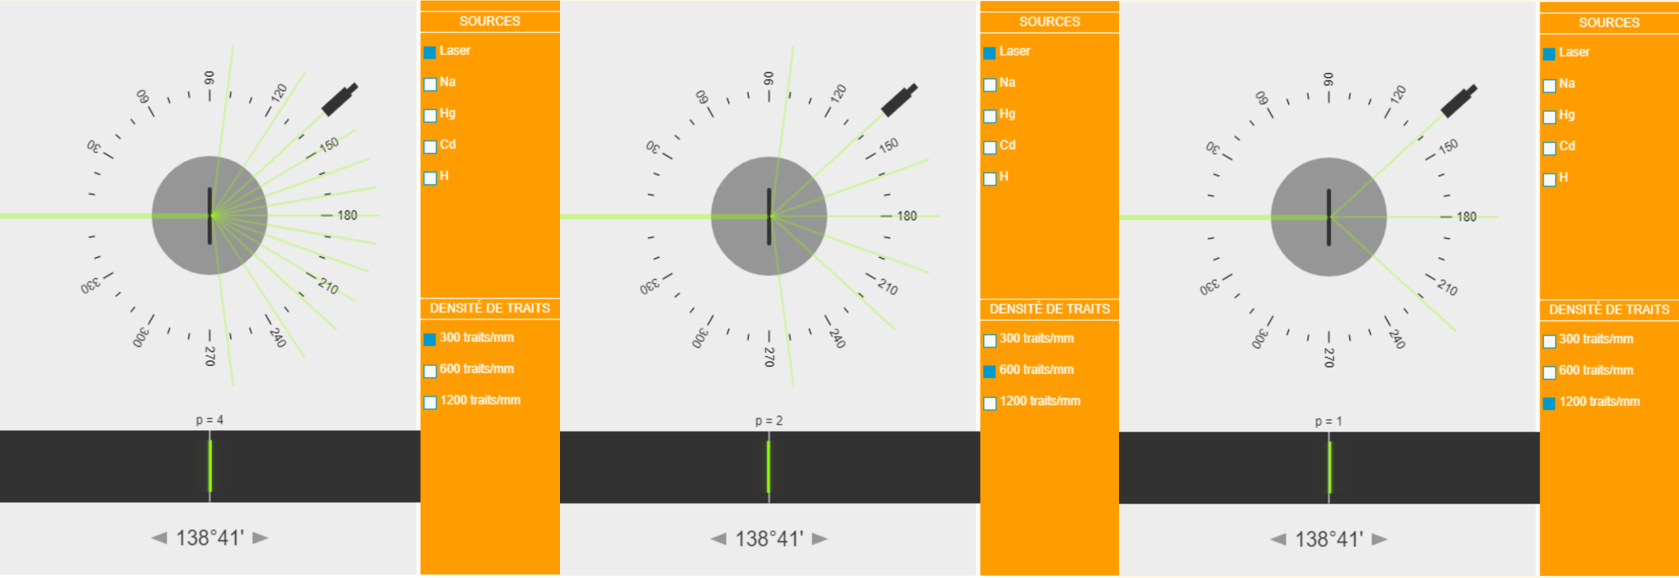
\includegraphics[scale=0.5]{tr131.png}
    \end{center}
    \caption{Changement de densité de traits(Lazer)}
\end{figure}
C'est le cas d'un incidence normale, par la formule des réseaux, on a donc $p\lambda_0=a\sin\theta_p$.
où $\theta_p$ est l'angle associé avec la maxima principal d'ordre $p$. 

On a donc $\boxed{p\frac{\lambda_0}{a}=\sin \theta_p \sim \theta_p}$ lorsque l'on fait l'observation dans les conditions de Gauss. 

Alors 
\begin{itemize}
    \item si $\lambda_0$ et $a$ sont constants, $\theta_p$ augment avec $p$
    \begin{figure}[h]
        \begin{center}
        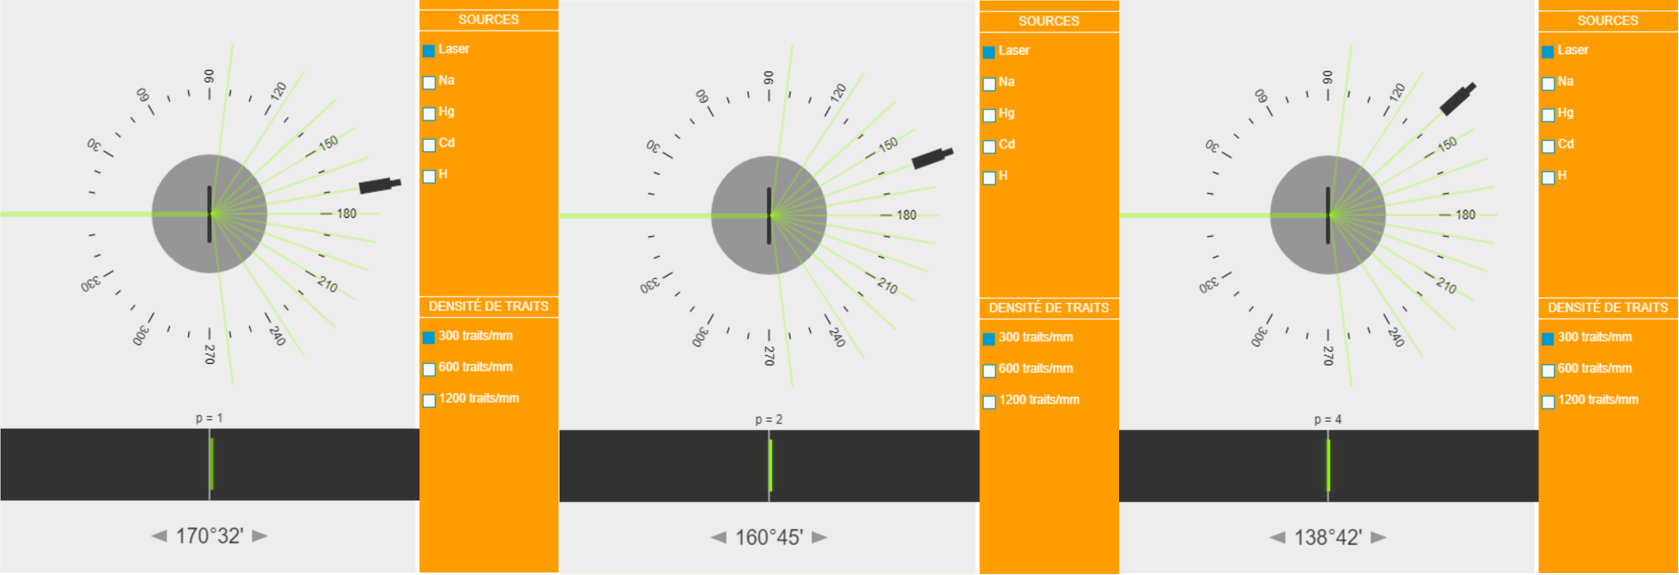
\includegraphics[scale=0.5]{tr132.png}
        \end{center}
        %\caption{Changement de densité de traits(Lazer)}
    \end{figure}
    \item si $\lambda_0$ et $p$ sont constants, $\theta_p$ diminue avec $a$ 
    \begin{figure}[h]
        \begin{center}
        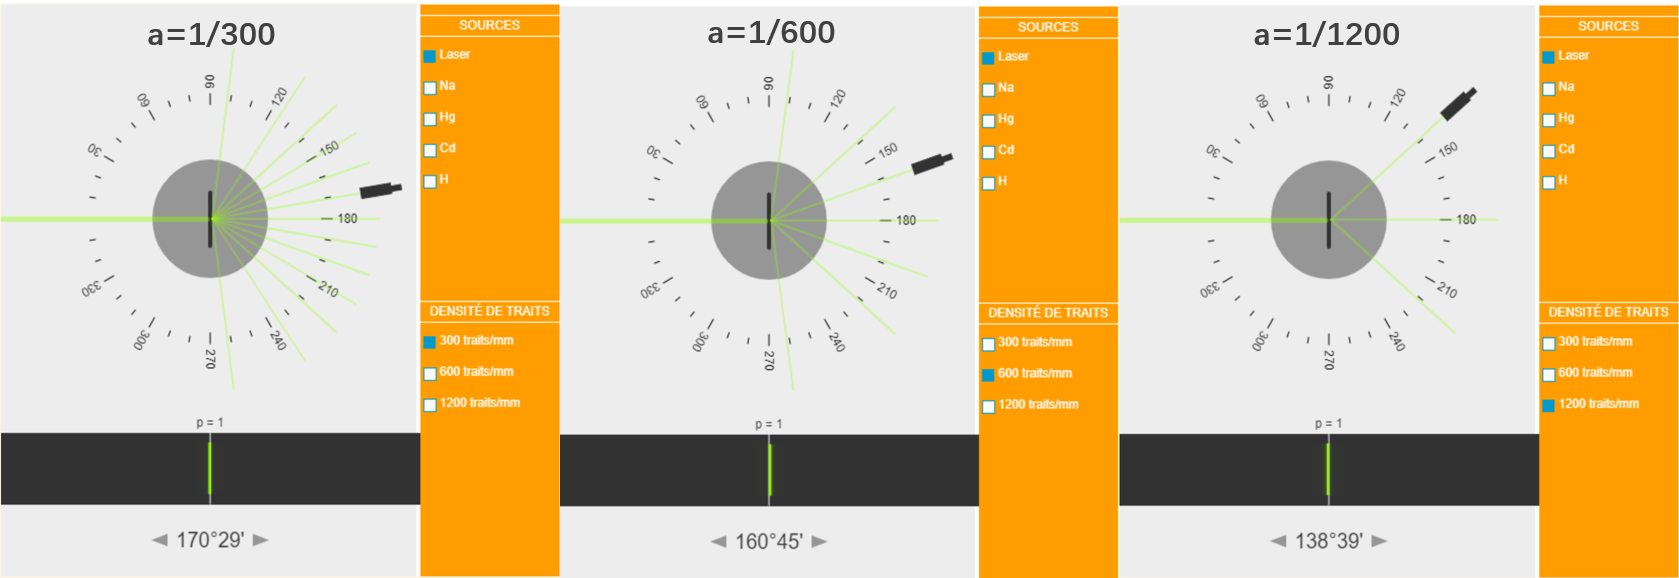
\includegraphics[scale=0.5]{tr133.png}
        \end{center}
        %\caption{Changement de densité de traits(Lazer)}
    \end{figure}   
    
    
    \item si $a$ et $p$ sont constants, $\theta_p$ augment avec $\lambda_0$
\end{itemize}
Si on fixe $\theta_p=138^\circ41^{'}$(voir Figure 1)s, on a $\boxed{\lambda_l=\frac{\theta_pa}{p}}$, avec $\frac{a}{p}=\frac{1}{1200}*10^{-3}=8.33*10^{-7}\,m$. 
A.N. $\boxed{\lambda_l=2.02*10^{-6}\,m}$, soit $202\,nm$ pour un Lazer

Et pour la lumière d'une lampe de $Na$, on a $\boxed{\lambda_{Na}=\frac{\theta_pa^{'}}{p}}$, avec $\frac{a^{'}}{p}=\frac{1}{1200}*10^{-3}=8.33*10^{-7}\,m$
A.N. $\boxed{\lambda_{Na}=\frac{134^\circ58^{'}}{180^\circ}*\pi*8.33*10^{-7}=1.96*10^{-6}\,m}$, soit $196\,nm$, plus court que celle d'un lazer.
\begin{figure}[h]
    \begin{center}
    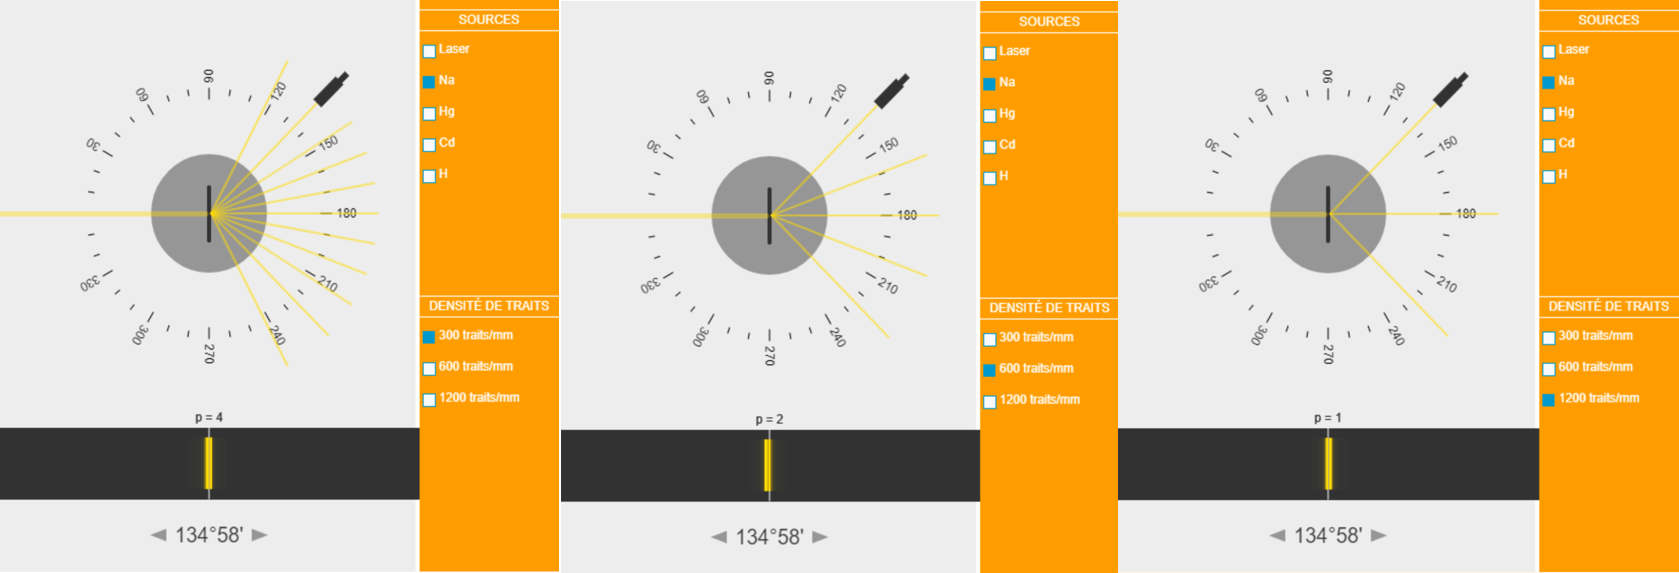
\includegraphics[scale=0.5]{tr134.png}
    \end{center}
    \caption{Changement de densité de traits(Na)}
\end{figure}  

On sait que le nombre d'ordres de diffraction observables est donné par $n=1+2\lfloor\frac{a}{\lambda_0}\rfloor$. 

Si on prend $a=8.33*10^{-7}\,m$, $\lambda_0=2.02*10^{-6}\,m$(voir la figure au-dessous), on a 
$n=1+\lfloor\frac{8.33*10^{-7}}{2.02*10^{-6}}\rfloor=1$, mais on peut observer $3$ ordres de diffraction sur la figure. 

Donc \fbox{la valeur obtenue n'est pas cohérente avec le nombre d’ordres de diffraction observables}
\begin{figure}[h]
    \begin{center}
    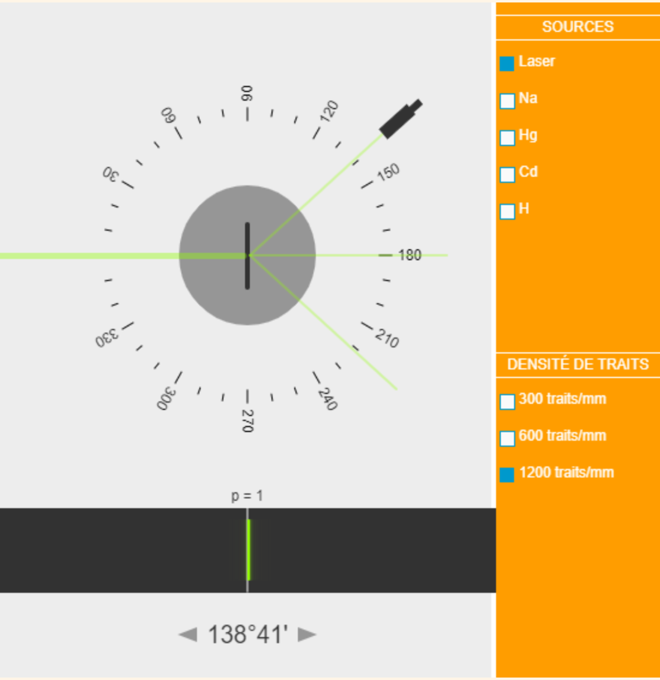
\includegraphics[scale=0.5]{tr135.png}
    \end{center}
    \caption{$a=8.33*10^{-7}\,m$ pour un lazer($\lambda_0=2.02*10^{-6}\,m$)}
\end{figure} 

\end{document}